This chapter, we examine the different \gls{MPES} datasets used throughout this study. We briefly discuss the data reduction and image formation pipeline, the characteristics of the datasets, and formation of target and noisy realizations. Beginning with how to evaluate the denoising performance, we move to applying the \gls{BM3D} algorithm with and without \gls{VST}. We apply a hyperparameter search to find the optimal $\sigma$ value for denoising, and evaluate the denoising performance across different count rates.

\section{Experimental Datasets}\label{section:datasets}
\subsection*{Datasets}
We investigate three datasets--\gls{GrIr} \cite{heberMultispectralTimeresolvedEnergy2022}, \gls{NiW} \cite{shokeenRealtimeObservationNonequilibrium2024}, and \gls{GdW} \cite{kutnyakhovMultidimensionalPhotoemissionSpectra2024}--that have been studied using \gls{HEXTOF} at \gls{FLASH}. Interpretable results from these experiments require long acquisition times (\gls{total_time}), essential for capturing the underlying physical processes. This is primarily due to three main reasons. 

As mentioned before, the intrinsic stochastic nature of the photoemission process requires the collection of a large number of events to approach the true value (expected value). Additionally, the low repetition rate of the \gls{FEL} means that the data  needs to be collected over a long period of time to get sufficient statistics. For example, as shown in \cref{fig:acq-time-1M}, acquiring $\gls{ncounts}=\num{e6}$ requires an acquisition time of $\gls{total_time}=\qty{8}{\min}$. Lastly, the multidimensional acquisition scheme to simultaneously resolve \gls{kx}, \gls{ky}, \gls{kz}, \gls{E}, \gls{tpp}, and spin polarization necessitates exponentially more data to adequately fill the sample space in higher dimensions.

\begin{figure}[h]
    \centering
    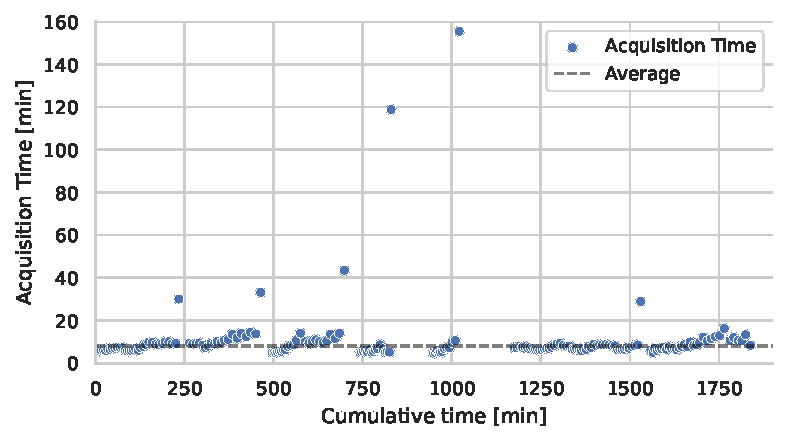
\includegraphics[width=0.8\linewidth]{images/acq_time_1M.pdf}
    \caption{Total acquisition time \gls{total_time} in minutes for generating \num{e6} data points. Some outliers are present due to the photon source being off, leading to longer \gls{total_time}. The average \gls{total_time} without outliers is approximately \qty{8}{min} (see dashed line).}
    \label{fig:acq-time-1M}
\end{figure}

For most of this study, we use the \gls{GrIr} dataset, as it features the longest acquisition time, and hence the highest number of counts, with $\gls{ncounts}=\num{1.86e8}$. The \gls{NiW} and \gls{GdW} datasets have comparatively lower total counts, at $\gls{ncounts}$ of \num{6.52e7} and \num{2.21e7}, respectively. 

However, \gls{ncounts} is not the only factor in determining data quality. Material-specific factors, sample conditions, and instrument settings can influence spectral clarity, meaning that a higher-count dataset does not necessarily guarantee more pronounced spectral features. For instance, while the \gls{NiW} dataset has a higher count rate than \gls{GdW}, its spectral features are comparatively less distinct as seen in \cref{fig:all-hextof-datasets-kxky}.

\begin{figure}[h]
    \centering
    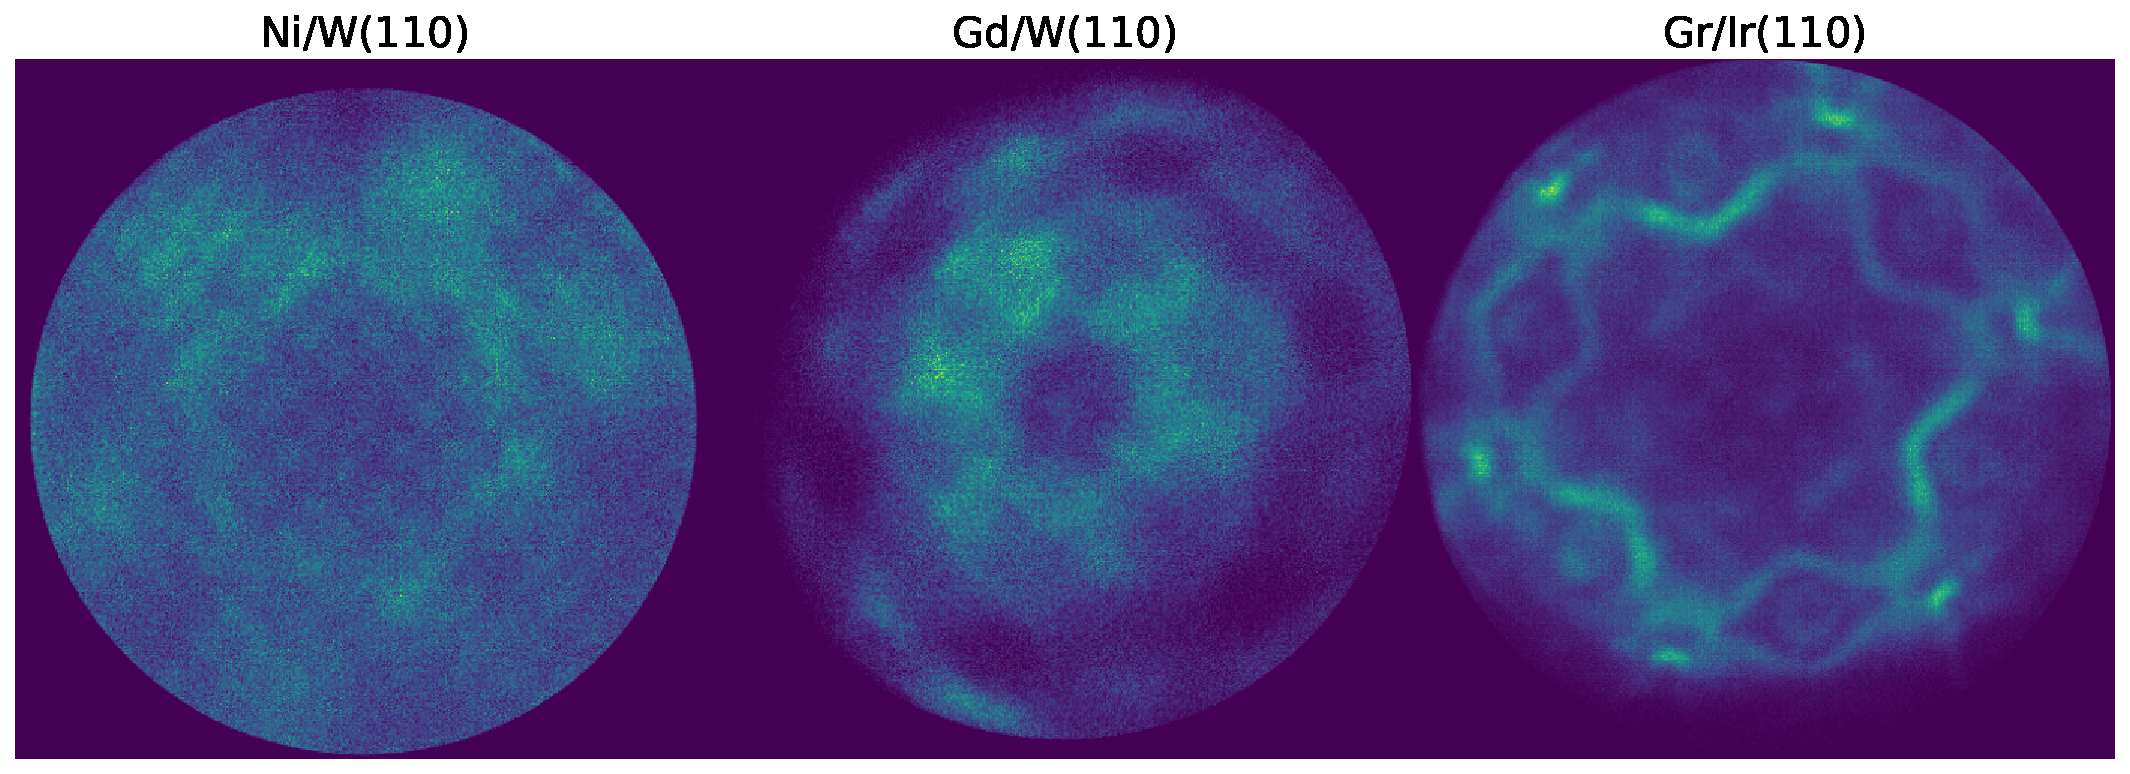
\includegraphics[width=1\linewidth]{images/datasets_3_kx_ky.pdf}
    \caption{A \gls{kx}-\gls{ky} slice of the \gls{GrIr}, \gls{NiW}, and \gls{GdW} datasets, window averaged across \gls{E} with $\gls{winsize}=\num{20}$.}
    \label{fig:all-hextof-datasets-kxky}
\end{figure}

For reference, we also look at the \gls{WSe2} dataset \cite{maklarTimeresolvedARPESRAW2022}, measured with a pulsed \gls{HHG}-based \gls{XUV} source with a \gls{TOF}-\gls{MM} analyzer. This dataset has a much larger number of counts, with $\gls{ncounts}=\num{e9}$, recorded in $\gls{total_time}=\qty{27}{s}$, compared to acquiring $\gls{ncounts}=\num{e6}$ in $\gls{total_time}=\qty{8}{\min}$ for the \gls{GrIr} dataset. The \gls{WSe2} dataset is used to compare the performance of denoising algorithms on a high-count dataset.

\subsection*{Constructing Image from Single-Event Data}
In an \gls{MPES} experiment using a \gls{TOF}-based scheme, the workflow to resolve images typically follows a series of steps, outlined in \cref{fig:mpes_workflow}. Prior to this, an essential step is data reduction, a detailed description\footnote{More specific to the \gls{HEXTOF} instrument at \gls{FLASH}.} of which is outlined in Appendix~\ref{sec:elt}.

After the data reduction, corrections are applied to the measurement axes e.g. to correct space-charge distortions (see \cref{section:spectroscopy-techniques}), correct timing jitter between \gls{FEL} and pump lase etc.. The corrected axes are then mapped (calibrated) to the physical axes, after which further correction steps can happen. Once calibrated, the single-event data is binned into a multidimensional volume\footnote{We make use of the Single Event DataFrame (SED) library \href{https://github.com/OpenCOMPES/sed}{https://github.com/OpenCOMPES/sed}.} that represents the full measurement, as illustrated on the right side of \cref{fig:mpes_workflow}.

\begin{figure}[h]
    \centering
    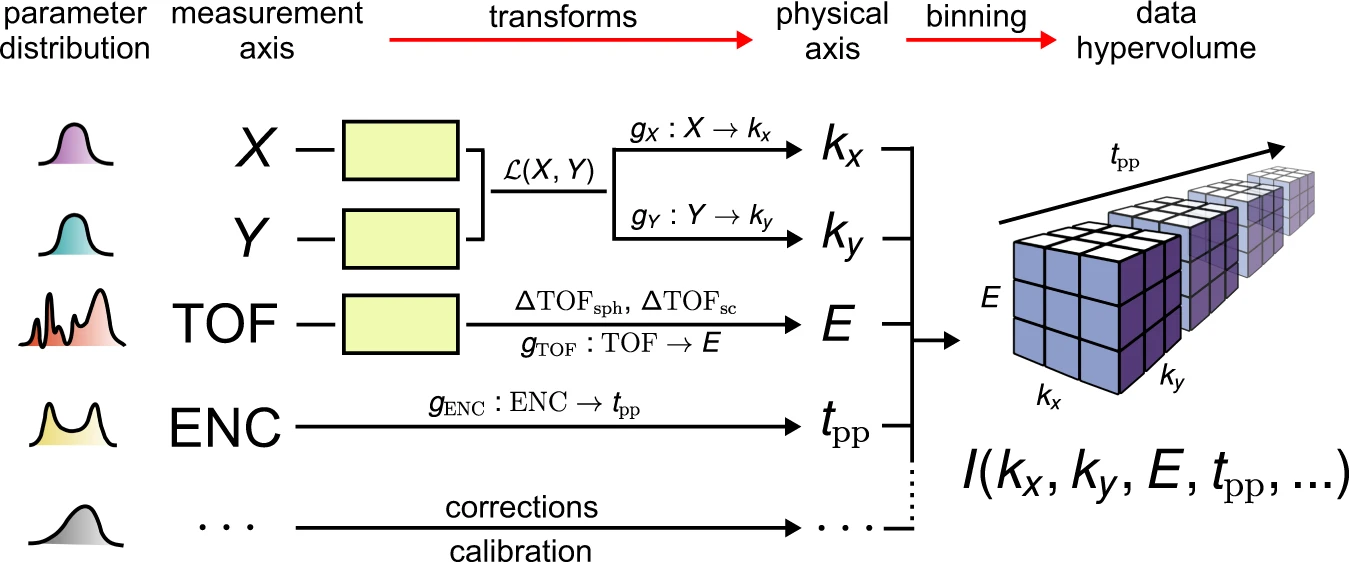
\includegraphics[width=1\linewidth]{images/41597_2020_769_Fig2_HTML.png}
    \caption{A typical workflow for an \gls{MPES} experiment, comprising transformations to the measured data and binning to form the multidimensional image. Reprinted from \cite{xianOpensourceEndtoendWorkflow2020}, under the terms of the Creative Commons Attribution 4.0 International License.}
    \label{fig:mpes_workflow}
\end{figure}

If we just look at the static spectra, a 3D image such as \cref{fig:3d-gr-ir} can be formed by binning across the three physical axes--\gls{kx}, \gls{ky} and \gls{E}--from different datasets such as the \gls{GrIr} dataset, containing \num{1.86e8} electron counts in the entire dataset. The average count decreases when binning across additional dimensions, such as the pump-probe time \gls{tpp} or spin polarization. After focusing on a region (\gls{EF} and near), and 3D binning with an image resolution of \qty{460}{px} in each direction, the total counts are \num{1.15e8}, with an average count of $\approx$\num{1.13} per voxel. Slicing along the \gls{E} direction, we can form 2D images such as already shown in \cref{fig:all-hextof-datasets-kxky}.

\begin{figure}[h]
    \centering
    \begin{subfigure}[t]{0.49\linewidth}
        \centering
        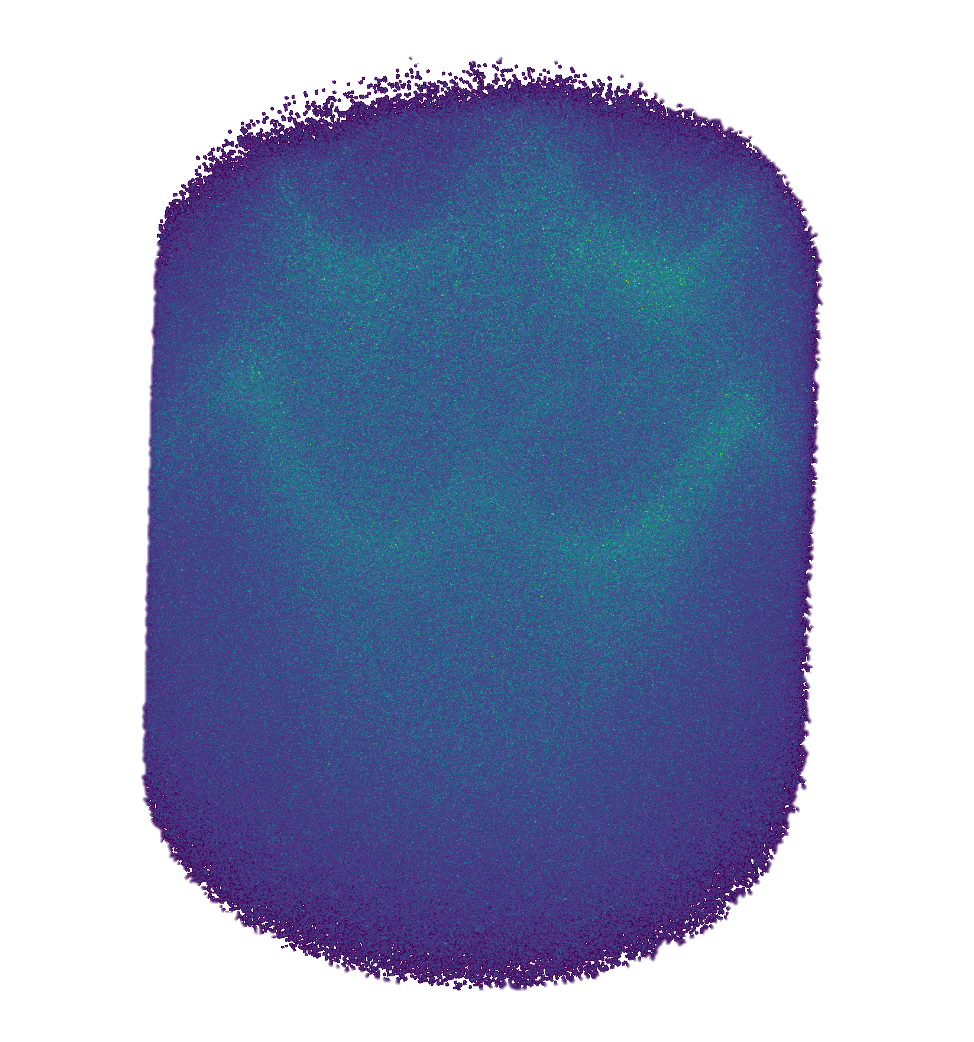
\includegraphics[width=1\linewidth]{images/3d_gr_ir_8M.png}
        \caption{$\gls{ncounts}=\num{8e6}$ corresponding to $\gls{total_time}=\qty{8}{min}$. The fine features of the data are not visible due to the low count rate.}
        \label{fig:3d-gr-ir-8M}
    \end{subfigure}
    \hfill
    \begin{subfigure}[t]{0.49\linewidth}
        \centering
        \includegraphics[width=1\linewidth]{images/3d_gr_ir_masked.png}
        \caption{$\gls{ncounts}=\num{1.86e8}$ corresponding to $\gls{total_time}=\qty{30}{hour}$. 2D images can be formed by slicing (or window averaging) along any of the axes, as depicted by the three lines.}
        \label{fig:3d-gr-ir-186M}
    \end{subfigure}
    \caption{3D images from the \gls{GrIr} dataset, with $\gls{ncounts}=\num{8e6}$ and \num{1.86e8}. The image is constructed by binning over the three physical axes $k_x$, $k_y$, $E$.}
    \label{fig:3d-gr-ir}
\end{figure}

\subsection*{Noisy Realizations}
With the \gls{DLD} providing a stream of single-event data, we are uniquely positioned to observe noisy realizations by taking subsets of varying electron counts \gls{ncounts} from the full dataset. These subsets can then be binned to form independent 3D images, used later for evaluating and training denoising algorithms.

For instance, from the complete dataset, \num{186} subsets, each with an \gls{ncounts} of \num{e6}, can be extracted. The data generation is assumed to be an \gls{iid} stochastic process, allowing for a large variety of randomly sampled subsets. However, due to the light source, which is not stable over extended periods, beyond its intrinsic fluctuations, sample degradation, temperature deviations and other reasons, this assumption is not entirely accurate.

\begin{table}[h!]
    \centering
    \resizebox{0.6\textwidth}{!}
        {%
        \begin{tabular}{lrrr}
            \toprule
            & \gls{ncounts} & Average Counts & $T$ [h] \\
            &  & Per Voxel & \\
            \midrule
            $n$ & \num{1e6} & \num{5.98e-3} & $\num{0.13}$ \\
            $2n$ & \num{2e6} & \num{1.22e-2} & $\num{0.28}$ \\
            $4n$ & \num{4e6} & \num{2.44e-2} & $\num{0.57}$ \\
            $8n$ & \num{8e6} & \num{4.89e-2} & $\num{1.23}$ \\
            $16n$ & \num{1.6e7} & \num{9.77e-2} & $\num{2.62}$ \\
            $32n$ & \num{3.2e7} & \num{2.00e-1} & $\num{5.32}$ \\
            $48n$ & \num{4.8e7} & \num{2.90e-1} & $\num{8.14}$ \\
            $96n$ & \num{9.6e7} & \num{5.84e-1} & $\num{16.07}$ \\
            $186n$ & \num{1.86e8} & \num{11.3e-1} & $\num{30.78}$ \\
            \bottomrule
        \end{tabular}
        }
    \caption{Table shows the noisy realizations generated by varying number of counts \gls{ncounts} from the \gls{GrIr} dataset. The acquisition time is proportional to \gls{ncounts} and $186n$ is used as the reference dataset.}
    \label{noisy-dataset-table}
\end{table}

Noisy realizations can then be formed based on different \gls{ncounts}. The total counts and average counts per voxel for each noisy realization are shown in \cref{noisy-dataset-table}. These realizations can help evaluate the performance of denoising algorithms as a function of \gls{total_time}. Lower count realizations ($\gls{ncounts}<\num{e7}$), corresponding to shorter \gls{total_time}, are of most interest to denoise. Successful denoising of such data--an example seen in \cref{fig:3d-gr-ir-8M}--could significantly improve experimental efficiency, allowing the investigators to steer the experiment in the right direction, crucial in time-limited \glspl{beamtime}. Hence, the realizations are sampled to cover a wide range of count rates, between \numrange{1e6}{1.86e8}.


\section{Denoising MPES data with BM3D}
As described in the last section, a 3D image is constructed by binning over the three physical axes $k_x$, $k_y$, $E$ from different datasets. By slicing along these axes, different 2D images can be generated for analysis. We evaluate the \gls{BM3D} algorithm, with and without the Anscombe transform\footnote{This was discussed in detail in \cref{ch:denoising}.}, using the \gls{GrIr} dataset, which has the highest average counts of all datasets. Despite this, the average voxel intensity is low (refer to \cref{noisy-dataset-table}), making a true, noise-free image unavailable. This limitation complicates the task of evaluating denoising performance, as standard metrics rely on comparison with such a noise-free reference.

\subsection{Evaluation Criteria}
Image quality assessment (IQA) is a field dedicated to measuring the objective and perpetual quality of an image. Objective metrics such as \gls{PSNR}, \gls{SSIM}, \gls{MSE} and \gls{MSSSIM} require a reference image\footnote{The metric definitions can be accessed in \cref{sec:metrics}.}---the latent clean image---to compare the denoised image against. No-reference metrics also exist, such as natural image quality evaluator (NIQE). However, these metrics are designed for real-world, non-scientific images. Subjective metrics such as the mean opinion score (MOS) can also be used, but these require evaluations by a group of experts, which can be impractical \cite{eskiciogluImageQualityMeasures1995,linzhangFSIMFeatureSimilarity2011}.

\begin{figure}
    \centering
    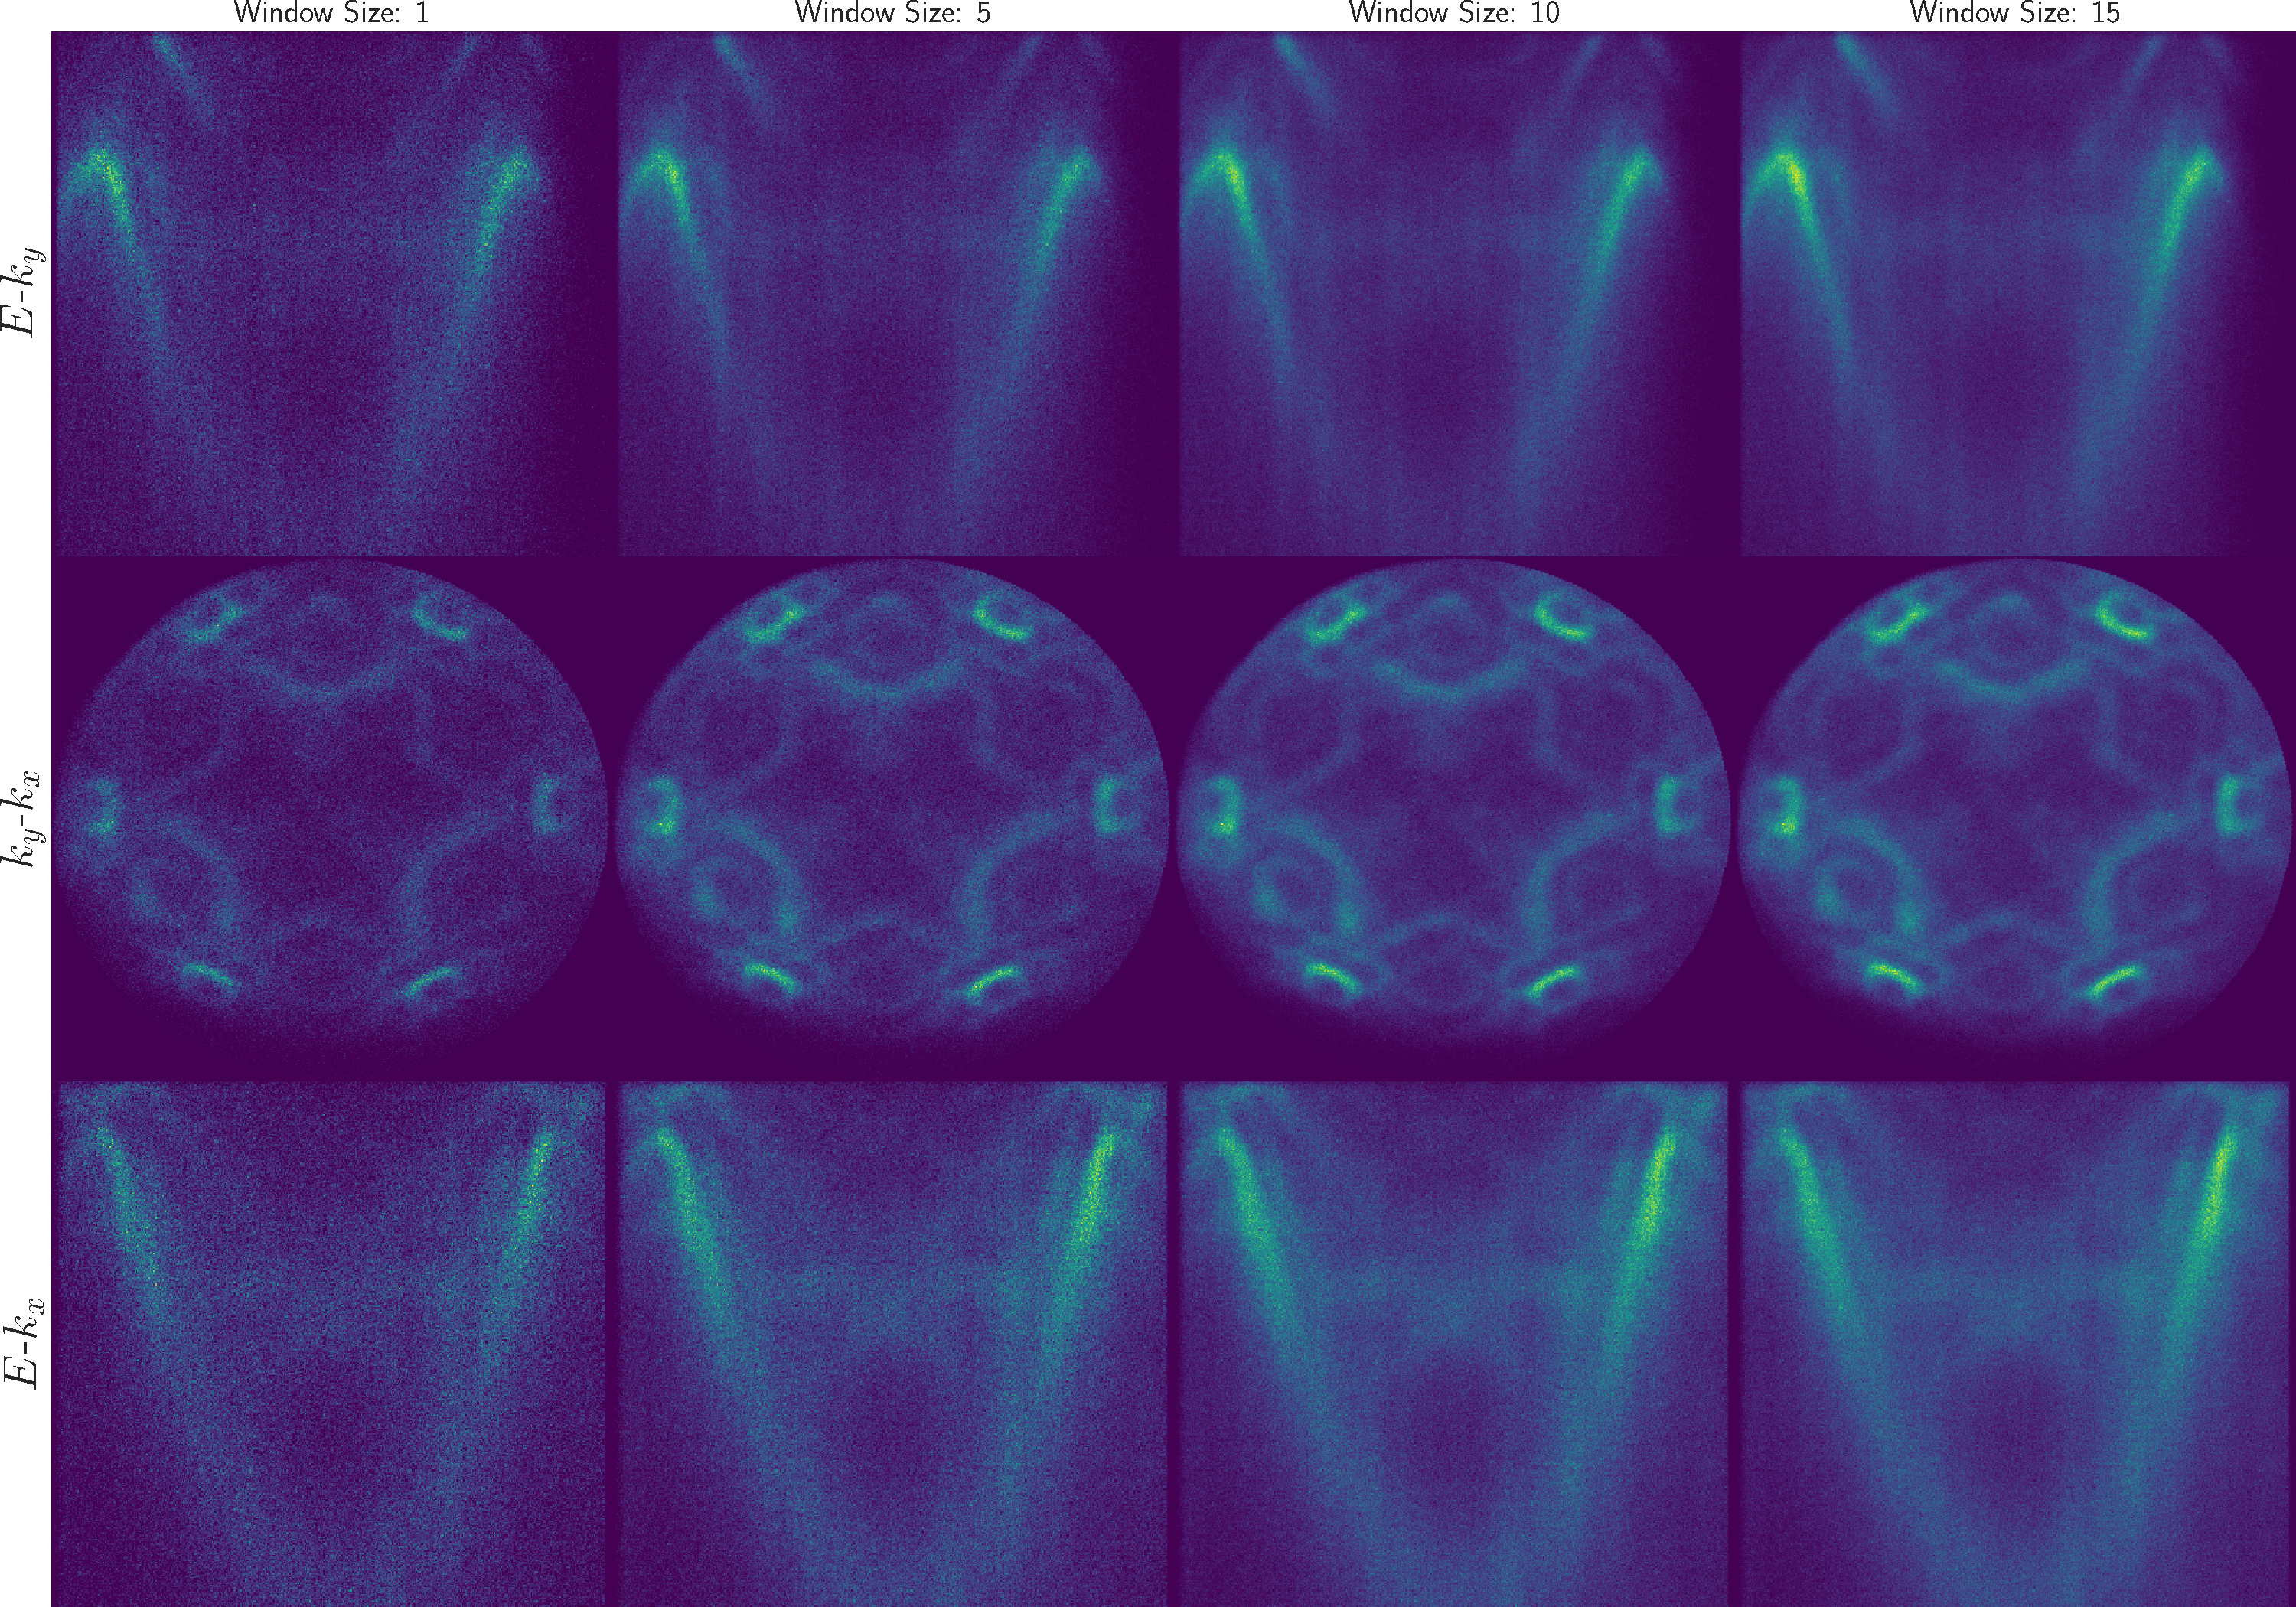
\includegraphics[width=1\linewidth]{images/slices.pdf}
    \caption{$E$, $k_y$, and $k_x$ slices at arbitrary positions of the \gls{GrIr} 3D dataset, showing the effect of averaging across different window sizes \gls{winsize}. The leftmost column shows a single slice ($\gls{winsize}=1$) with significant noise, while subsequent columns show window-averaged images with $\gls{winsize}=\numlist{5;10;15}$. Increasing \gls{winsize} progressively reduces noise, at the cost of feature broadening. This trade-off highlights the difficulty in obtaining a true, noise-free reference image even through averaging techniques.}
    \label{fig:slices}
\end{figure}

Given the low \gls{ncounts} in the dataset, a possible method to create a higher quality reference image is to window-average across neighboring slices. \cref{fig:slices} illustrates such a case, where noise is progressively reduced by averaging across windows of increasing size (see \cref{fig:3d-gr-ir} for a 3D depiction of slice axis), at the cost of feature blurring. Even with a large window size, an ideal, noise-free reference image is not obtainable.

To address this, we assess metrics that are more resilient to noisy reference images. In \cref{sec:metric_comparison_experiment}, we compare the performance of different metrics (\gls{PSNR}, \gls{SSIM}, \gls{MSE} and \gls{MSSSIM}) for evaluating the denoising performance. Our findings suggest that the \gls{MSSSIM} metric is particularly well-suited for evaluating the denoising performance of images, when comparing against a noisy reference image. The \gls{MSSSIM} metric, conceived by \citeauthor{wangMultiscaleStructuralSimilarity2003} \cite{wangMultiscaleStructuralSimilarity2003}, extends SSIM by incorporating multiple scales. 

Given that the ideal denoising aims to produce distortion-free images, one free from artifacts and removing all unwanted signal, it makes sense to target structural similarity rather than relative intensity values against the reference. Hence, throughout this study, the images are normalized to the [\num{0}, \num{1}] range. This normalization ensures that comparisons focus on relative differences in image structures and features, rather than on absolute intensity values.

Let us start with attempting to denoise the noisy realization with $\gls{ncounts}=\num{1.6e7}$ ($\gls{total_time}\approx\qty{2}{h}$) of the $k_y$-$k_x$ images shown in \cref{fig:slices}. This particular slice serves as a good reference due to its clear features. We use the Anscombe--\gls{BM3D}--Inverse Anscombe scheme described in \cref{alg:anscombe-bm3d}. The noisy image is formed by window-averaging along the $E$ dimension with window size $w = 5$. The respective denoised image is compared against the reference image (with $w=15$) of $\gls{ncounts}=\num{1.86e8}$, using the \gls{MSSSIM} metric. An example noisy, denoised and target set is shown in \cref{fig:noisy-denoised-ref-16M-avg-bm3d}. 

\begin{figure}
    \centering
    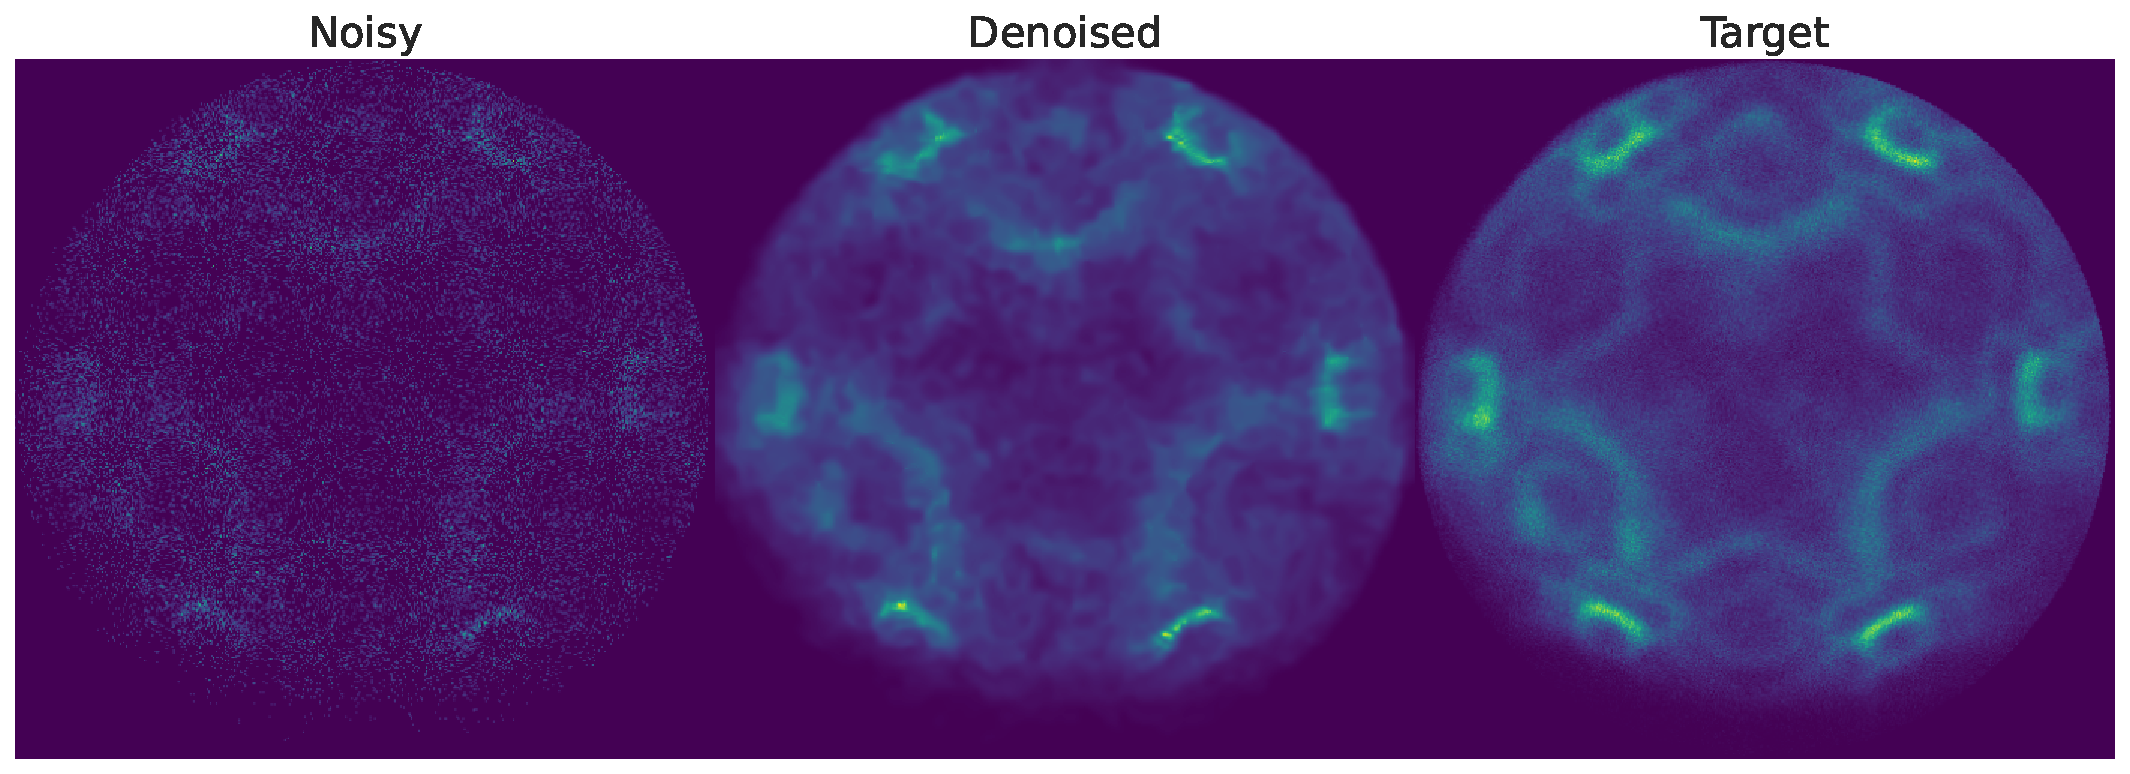
\includegraphics[width=1\linewidth]{images/noisy_denoised_ref_16M_avg_bm3d.pdf}
    \caption{Noisy, denoised, and target images. The noisy and target images are window-averaged with size $w=5$ and $w=15$ along the $E$ dimension, respectively.}
    \label{fig:noisy-denoised-ref-16M-avg-bm3d}
\end{figure}

\subsection{Single and Window-Averaged Images}
The above-mentioned evaluation is now repeated by varying $w = \numlist{1;5;10;15}$ for both noisy and target images. \cref{fig:confusion_matrix_msssim_window_avg} presents a confusion matrix that shows how the metric varies when $w$ is varied. It becomes evident that a larger $w$ yields a better comparison for denoising. This is because a larger $w$ reduces the noise in the target image, leading to a more accurate evaluation.

\begin{figure}
    \centering
    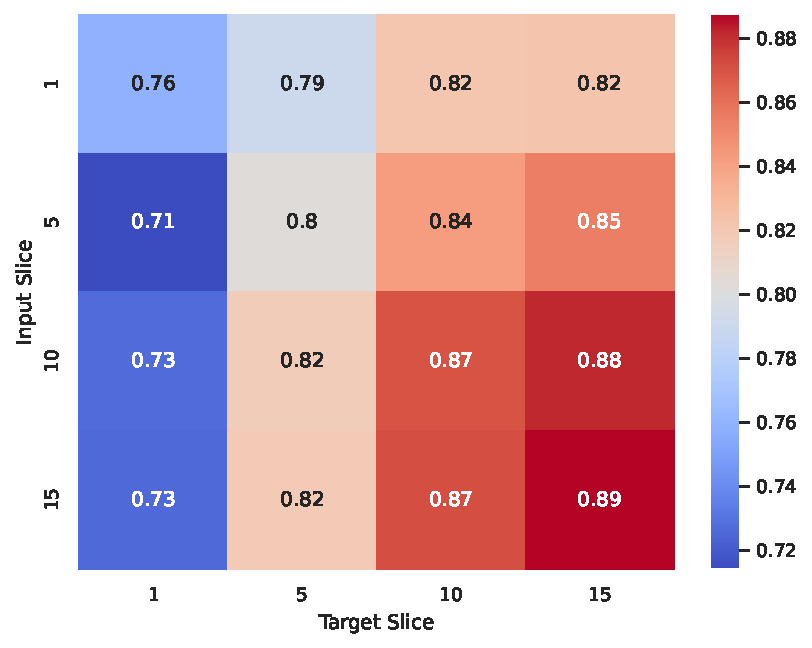
\includegraphics[width=0.5\linewidth]{images/confusion_matrix_msssim_window_avg.pdf}
    \caption{Confusion matrix showing the \gls{MSSSIM} values with different windows $w$ for input and target images. The \gls{MSSSIM} is computed for the denoised images using \cref{alg:anscombe-bm3d}. The matrix shows that using a larger $w$ for target image leads to better comparison of denoising.}
    \label{fig:confusion_matrix_msssim_window_avg}
\end{figure}

\subsection{Finding the Optimal Sigma}
\begin{figure}
    \centering
    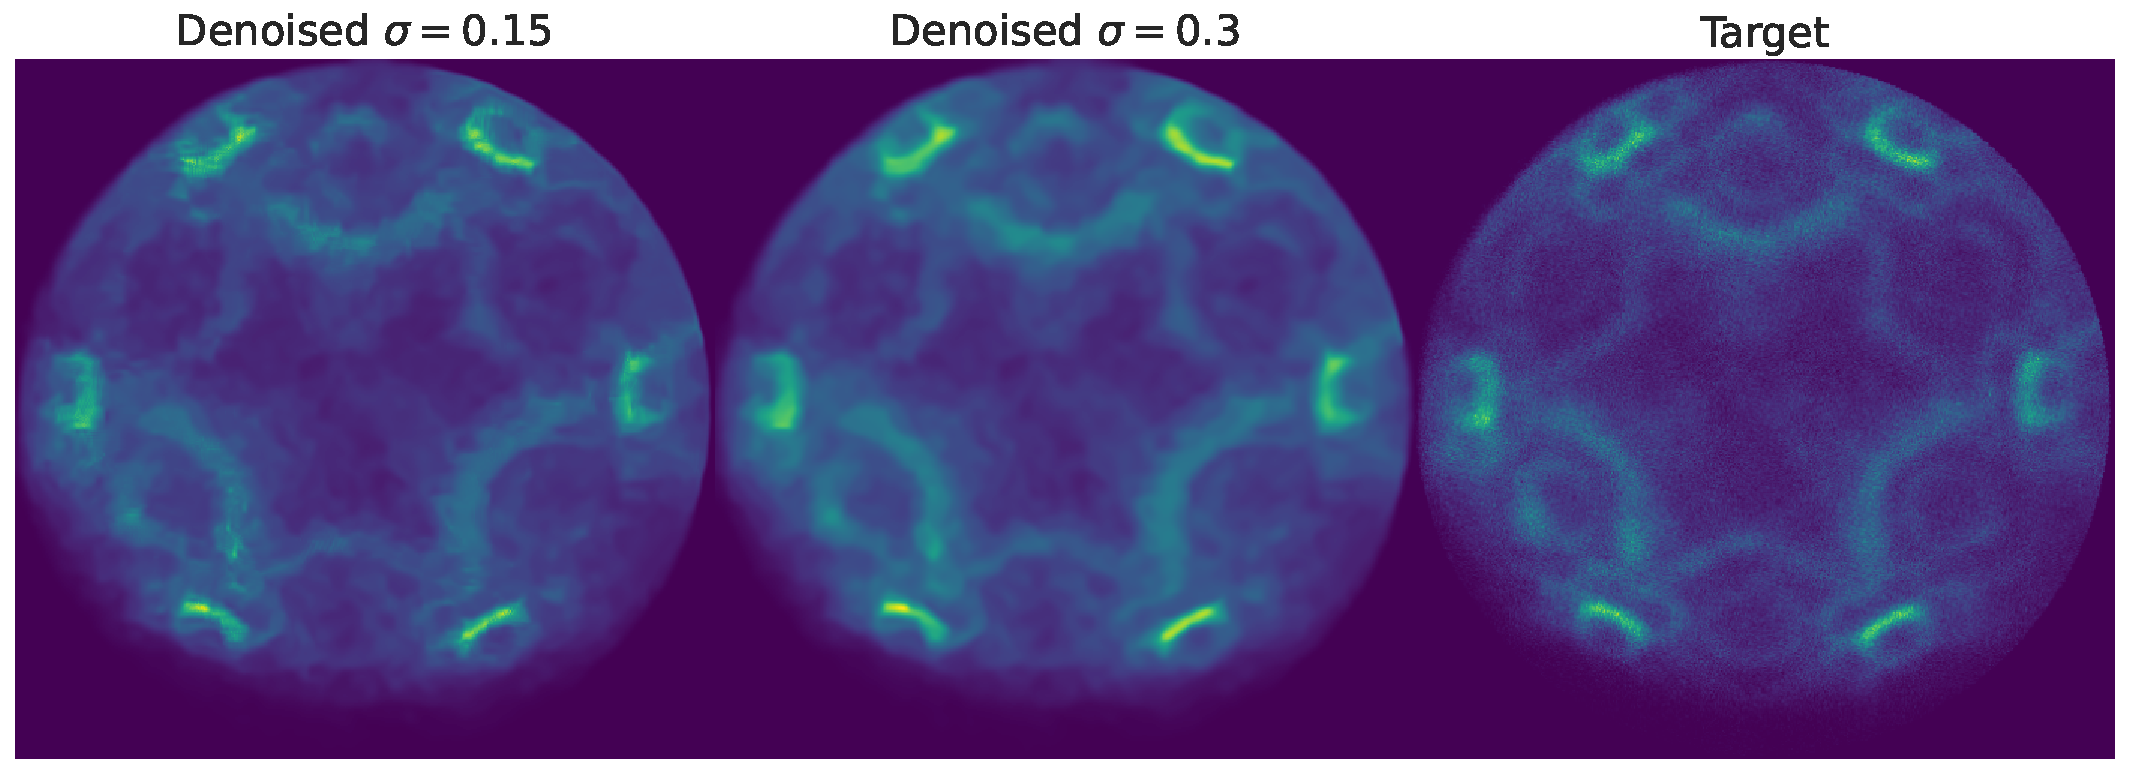
\includegraphics[width=1\linewidth]{images/denoised_optimal_sigma.pdf}
    \caption{Denoised image using the optimal $\sigma_{\text{oo}}=0.15$ (optimal value found for \num{1.6e7} counts from the hyperparameter search) denoised image with $\sigma_{\text{o}}=0.3$ (adjusted optimal value) and the target image.}
    \label{fig:denoised-optimal-sigma}
\end{figure}
Till now, we only focused on a single count rate and applied denoising with a single $\sigma$ value. However, considering that the noise decreases with increased electron counts, we would expect the required level of denoising to decrease i.e. $\gls{ncounts}\propto\frac{1}{\sigma}$.

One way to find the optimal denoising strength would be to estimate the noise level and use that estimate as the $\sigma$ for denoising. A different approach would be to perform a constrained optimization to find optimal $\sigma$ denoted $\sigma_{\text{oo}}$, such that the metric \gls{MSSSIM} is maximized. For user defined parameters to an algorithm, this sort of optimization is known as a hyperparameter search. An exhaustive grid search is the simplest method, but it is computationally expensive. Therefore, we use \texttt{optuna}\footnote{\href{https://optuna.org/}{https://optuna.org/} see citation in acknowledgments.}, which performs Bayesian optimization to find the optimal parameters, optimizing for \num{50} trials.

The search is conducted on a small set of \num{2} identical featured images, featuring the same characteristics as shown in \cref{fig:noisy-denoised-ref-16M-avg-bm3d}, using a window size of ($\gls{winsize} = \num{10}$) across the count range of \numrange{1e6}{4.8e7}. The values of $\sigma$ are constrained between \numrange{0}{5} to prevent the disappearance of features, as higher values can lead to significant loss of detail. The results in \cref{fig:hyperparameter-averaged-10-images} corroborate the hypothesis that the optimal $\sigma$ for denoising decreases with increasing electron counts, a linearly decreasing trend.

\begin{figure}
    \centering
    % First subfigure (Hyperparameter Search with Averaged 10 Images using MS-SSIM)
    \begin{subfigure}[t]{0.49\linewidth}
        \centering
        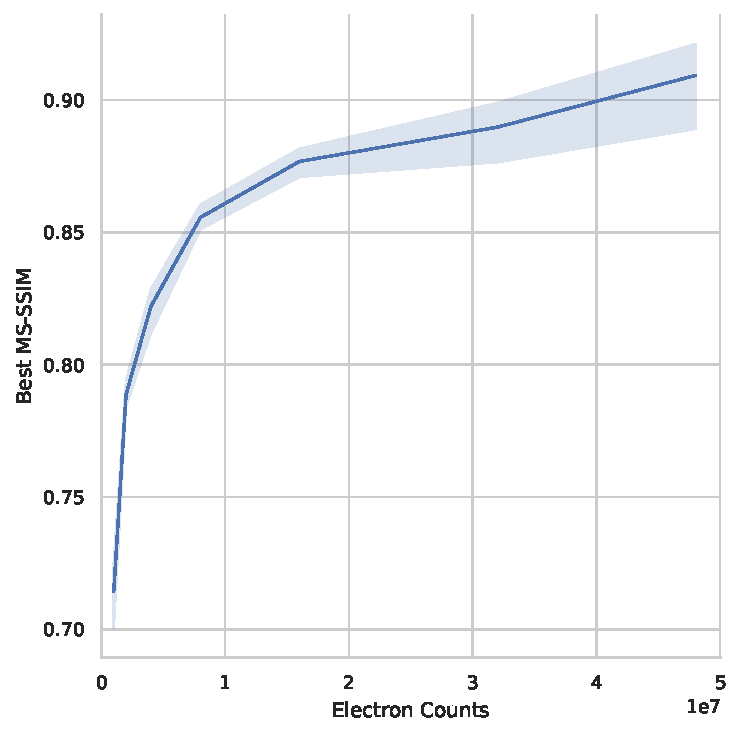
\includegraphics[width=\linewidth]{images/hyperparameter_msssim_averaged_10_images.pdf}
        \caption{Hyperparameter search results using MS-SSIM metric, averaged over 10 images.}
        \label{fig:hyperparameter-msssim-averaged-10-images}
    \end{subfigure}
    \hfill
    % Second subfigure (Hyperparameter Search with Averaged 10 Images using Sigma)
    \begin{subfigure}[t]{0.49\linewidth}
        \centering
        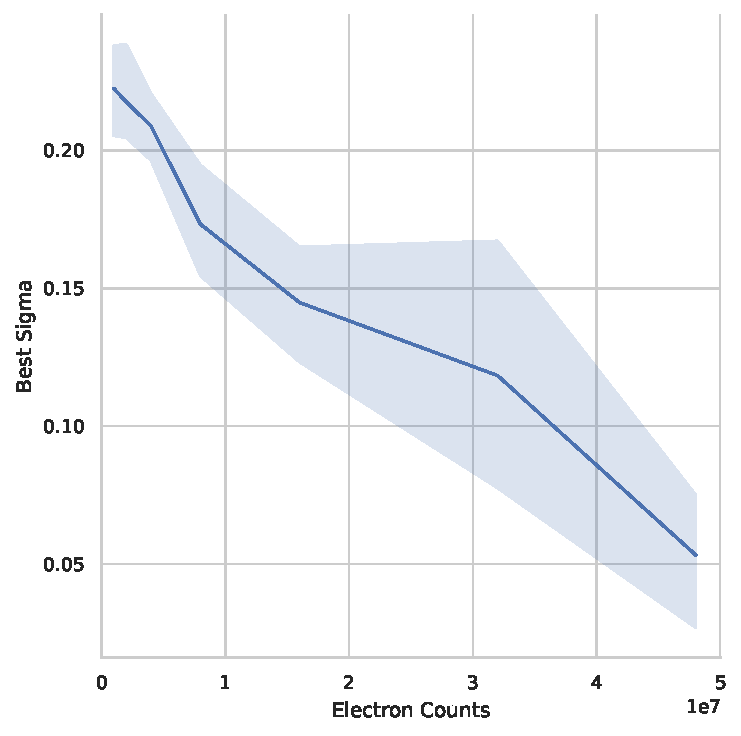
\includegraphics[width=\linewidth]{images/hyperparameter_sigma_averaged_10_images.pdf}
        \caption{Hyperparameter search results using Sigma metric, averaged over 10 images.}
        \label{fig:hyperparameter-sigma-averaged-10-images}
    \end{subfigure}
    \caption{Results of hyperparameter search for \gls{BM3D} $\sigma$ for different electron counts, using the \gls{MSSSIM} metric. The images are a window-average of \num{10} slices from the 3D volume.}
    \label{fig:hyperparameter-averaged-10-images}
\end{figure}

While using \gls{MSSSIM} as the objective function for optimization is good at showing the denoising performance improvement, it leads to more cautious results (low $\sigma_{\text{oo}}$ values) as those fare better against the target, which has the relevant features but is also noisy. To counter that, we scale the optimum $\sigma_{\text{oo}}$ values by a factor of 2 to get a more aggressive denoising and denote that as $\sigma_{\text{o}}$ and use this for denoising. A comparison of the denoised image using the optimal $\sigma_{\text{o}}$ and the adjusted optimal $\sigma_{\text{oo}}$ is shown in \cref{fig:denoised-optimal-sigma}.

The denoising performance below \num{4e6} is poor, with or without the optimal value $\sigma_{\text{oo}}$, even though the \gls{MSSSIM} reports high values. \cref{fig:noisy-denoised-ref-2M-avg-bm3d} and \cref{fig:noisy-denoised-ref-4M-avg-bm3d} show the denoised images for \num{2e6} and \num{4e6} counts, with an average count of \num{0.14} and \num{0.27} in the noisy image, respectively, whereas the average count in target image is \num{12.9}. It can be seen that the perpetual quality of the denoised images is poor, with the features not being well-preserved. This highlights that \gls{BM3D} is not well suited for denoising such low count images.

\begin{figure}
    \centering

    \begin{subfigure}[b]{1\linewidth}
        \centering
        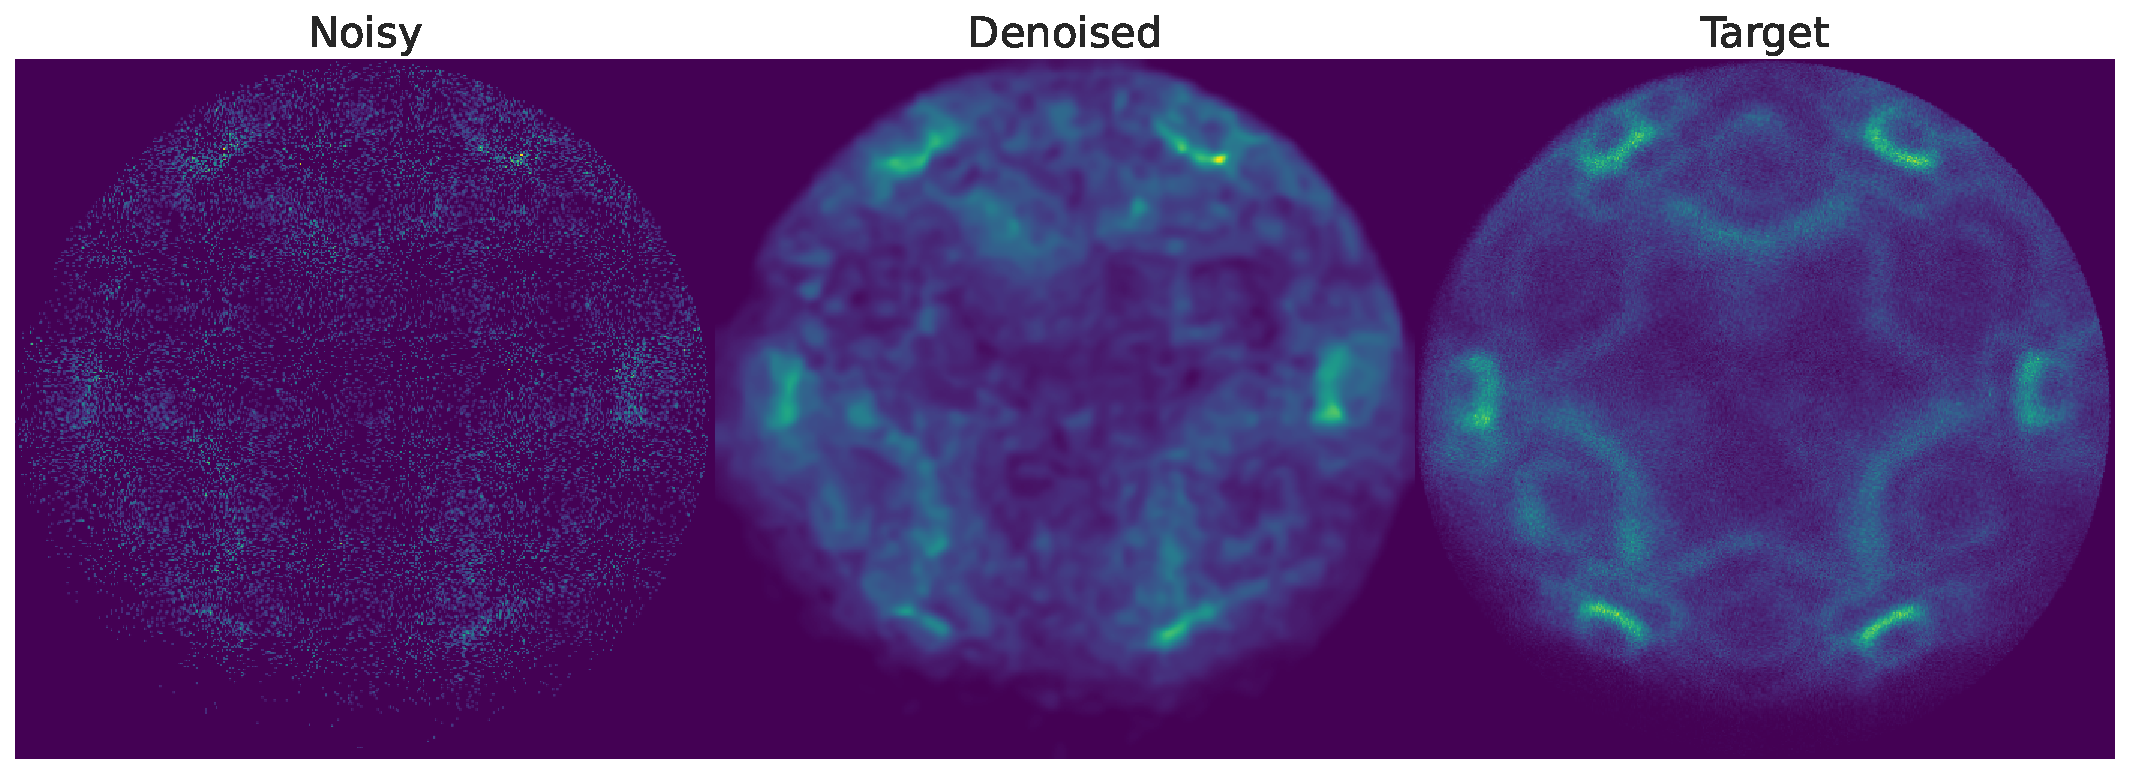
\includegraphics[width=1\linewidth]{images/noisy_denoised_ref_2M_avg_bm3d.pdf}
        \caption{Dataset with $\gls{ncounts}=\num{2e6}$. The denoising performance is quite poor, even with the adjusted optimal $\sigma_{\text{o}}\approx0.4$.}
        \label{fig:noisy-denoised-ref-2M-avg-bm3d}
    \end{subfigure}

    \begin{subfigure}[b]{1\linewidth}
        \centering
        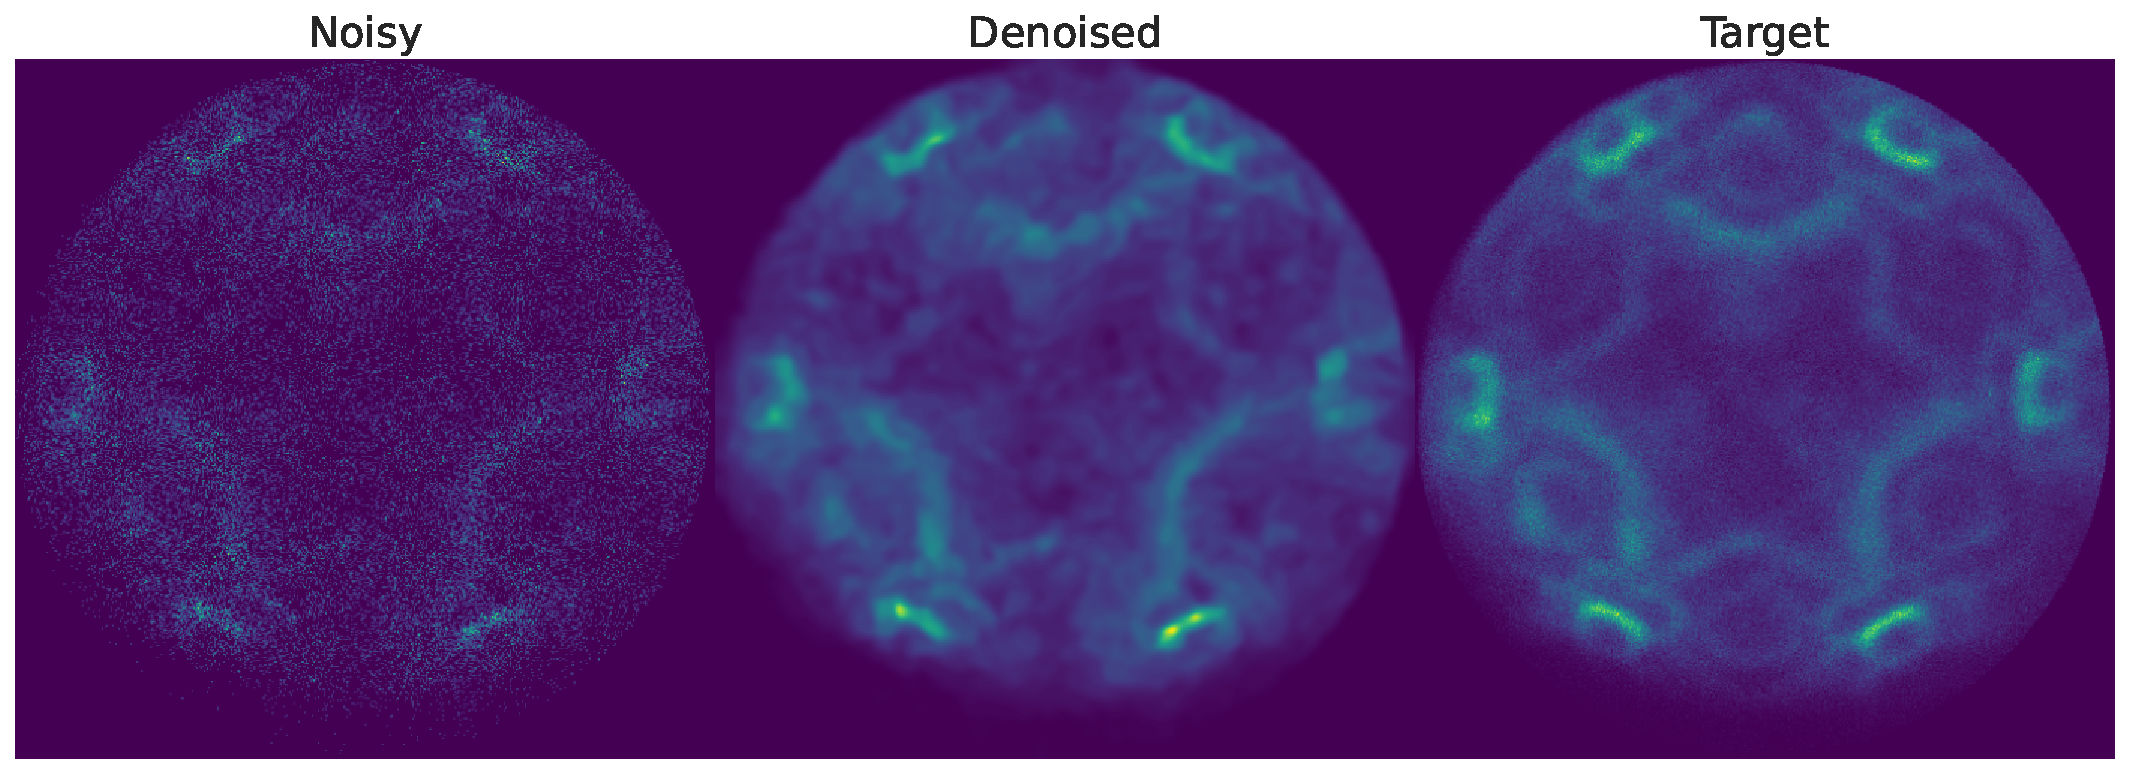
\includegraphics[width=1\linewidth]{images/noisy_denoised_ref_4M_avg_bm3d.pdf}
        \caption{Dataset with $\gls{ncounts}=\num{4e6}$. The denoising performance leaves room for improvement, using the adjusted optimal $\sigma_{\text{o}}\approx0.4$.}
        \label{fig:noisy-denoised-ref-4M-avg-bm3d}
    \end{subfigure}

    \begin{subfigure}[b]{1\linewidth}
        \centering
        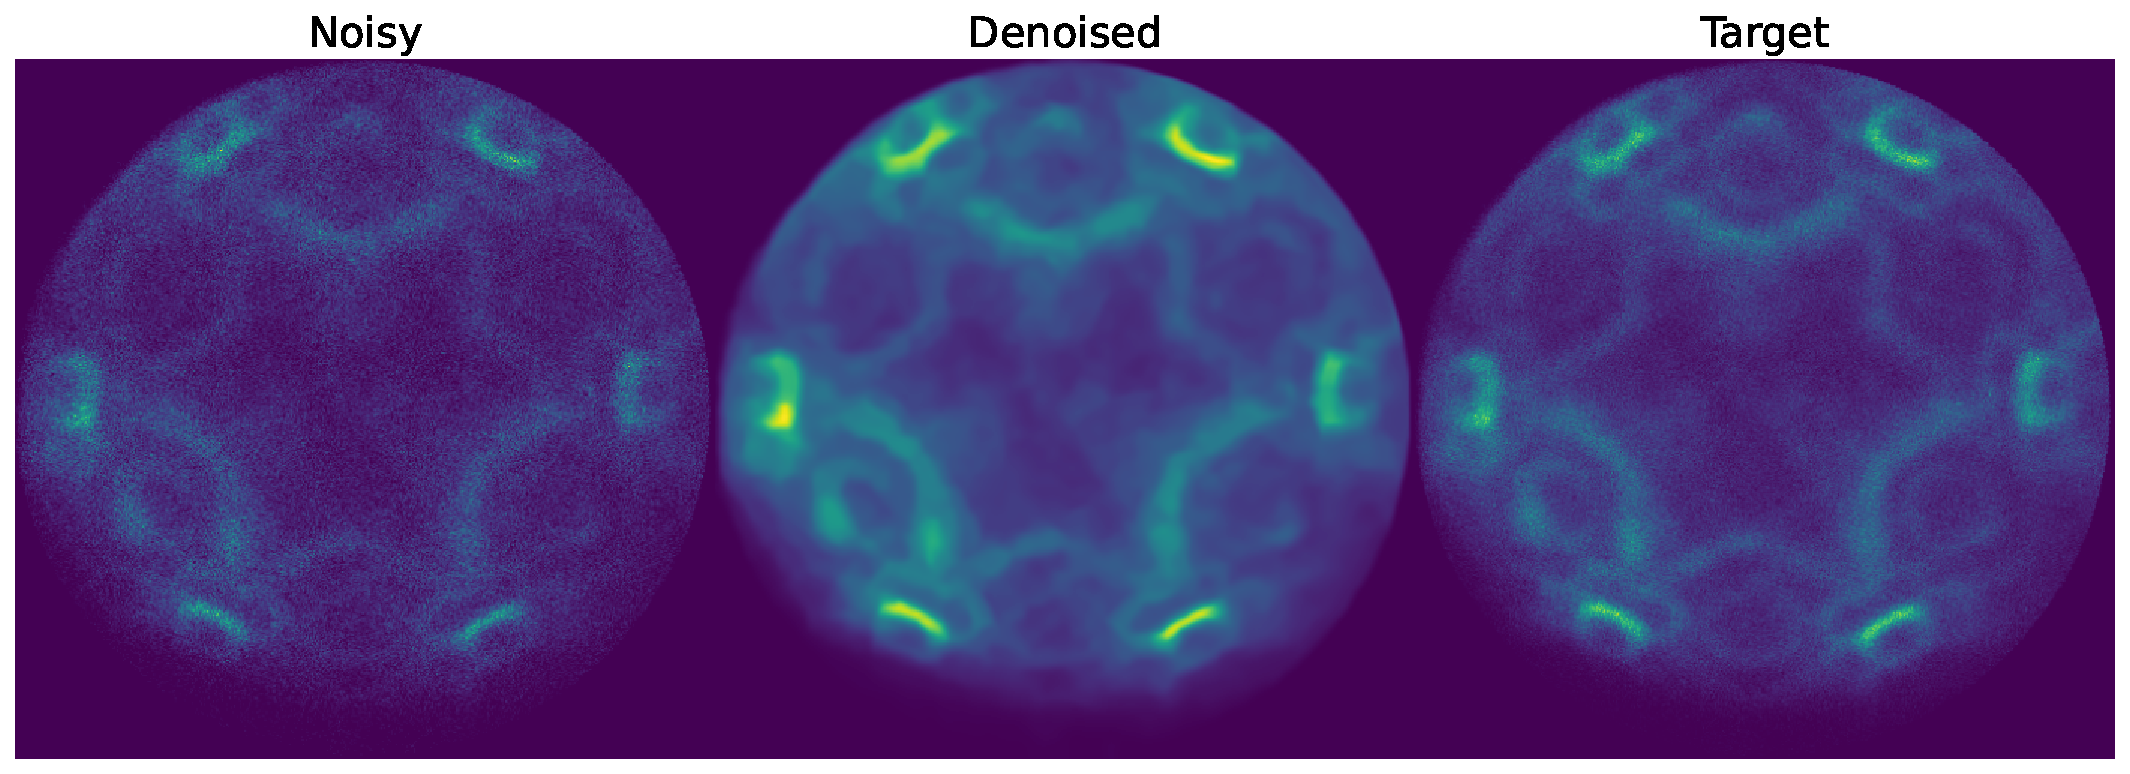
\includegraphics[width=1\linewidth]{images/noisy_denoised_ref_48M_avg_bm3d.pdf}
        \caption{Dataset with $\gls{ncounts}=\num{4.8e7}$. At this count rate, \gls{MSSSIM} reports lower values for the denoised images compared to the noisy images, even though the denoised image features are well-preserved.}
        \label{fig:noisy-denoised-ref-48M-avg-bm3d}
    \end{subfigure}

    \caption{Comparison of noisy, denoised, and target images for $\gls{ncounts}=$\numlist{2e6;4e6;4.8e7}, where the noisy and target images were formed using with $\gls{winsize}=\num{10}$ over \gls{E} to form \gls{kx}-\gls{ky} images. The \gls{BM3D} algorithm with Anscombe transform (\cref{alg:anscombe-bm3d}) was used for denoising.}
    \label{fig:combined-noisy-denoised}
\end{figure}

\subsection{Varying Total Counts}
We now evaluate the denoising performance of \cref{alg:anscombe-bm3d} (\gls{BM3D} with Anscombe) and \cref{alg:bm3d} (\gls{BM3D} without Anscombe), using the optimal $\sigma_{\text{o}}$ values determined through the hyperparameter search. A total of \num{1847} images were extracted from two separate noisy realizations of $\gls{ncounts}=\numlist{1e6;2e6;4e6;8e6;1.6e7;3.2e7;4.8e7}$. These are window-averaged with $\gls{winsize}=10$ for both the noisy and target images. 

As before, the \gls{MSSSIM} metric is used, with the baseline computed using the noisy images. Averaging over the large amount of images at varied counts gives us a robust estimate of the denoising performance. Using statistical bootstrapping, where the estimate is computed over multiple resamples of the data, we can also estimate the \num{95}\% confidence interval of the \gls{MSSSIM} metric.

As shown in \cref{fig:bm3d-msssim}, there is a noticeable improvement in image quality with counts up to $\gls{ncounts}=\num{4e7}$, with \gls{MSSSIM} values increasing from \num{0.6} to \num{0.83}. Beyond this count, the metric starts reporting lower values for denoised results, and visual inspection reveals that the denoised images contain similar information as the target, just smoother with preserved features. We can see this in \cref{fig:noisy-denoised-ref-48M-avg-bm3d}, where the denoised image has a lower \gls{MSSSIM} value compared to the noisy image, but the features are well-preserved.

\begin{figure}
    \centering
    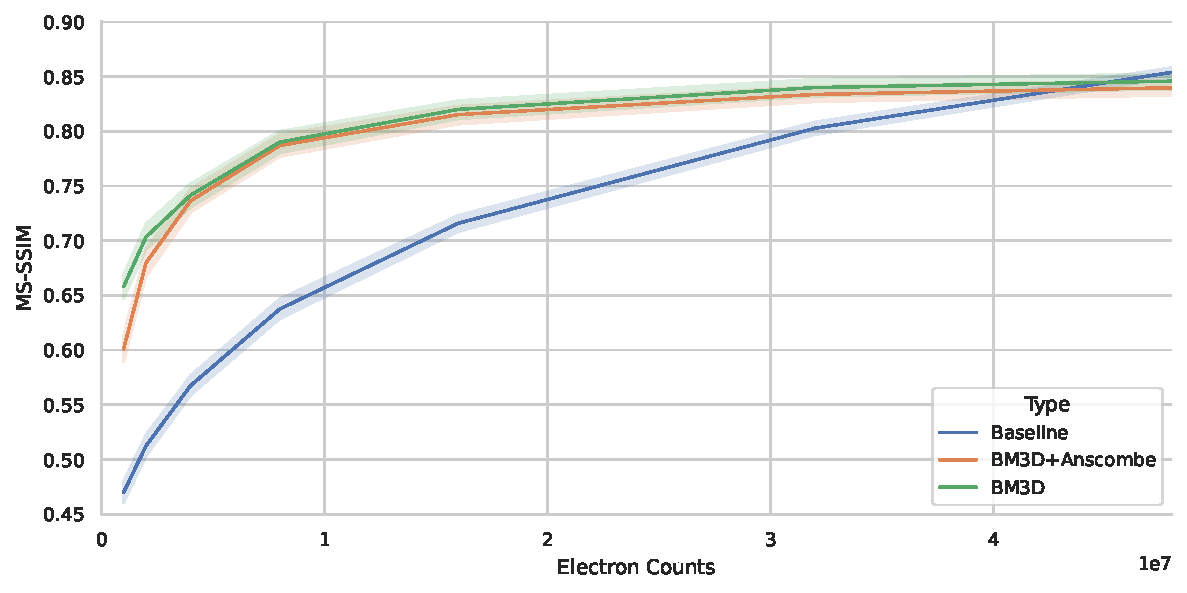
\includegraphics[width=1\linewidth]{images/bm3d_msssim.pdf}
    \caption{Denoising performance of the \gls{BM3D} algorithm, with and without the Anscombe transformation. The optimal $\sigma_{\text{o}}$ values determined through the hyperparameter search are used. The images are window-averaged with $\gls{winsize}=10$ slices for both the noisy and target images. The baseline metric is computed using the noisy image as input.}
    \label{fig:bm3d-msssim}
\end{figure}


The most notable finding is that the application of the \gls{VST} leads to a slightly worse performance (\cref{fig:bm3d-msssim} orange vs. green lines), despite the expectation that it would enhance denoising performance for Poissonian noise. In previous work by \citeauthor{makitaloOptimalInversionAnscombe2011}, the authors demonstrated that applying the Anscombe transform indeed improves denoising performance. This strongly suggests that the noise statistics in the image deviate from a Poisson distribution. This shall be the topic of the next chapter. 
